% Final report (v4) = the frozen v3 report + the post-hoc Phase-4 section (Sec. VII).
% Build: .venv/bin/python scripts/final_report_v4.py && cd report/final_v4 && tectonic final_report_v4.tex
% v3 numbers: generated/macros.tex + t_*.tex (scripts/final_report_v3.py, copied unchanged);
% Phase-4 numbers: generated/macros_v4.tex + t_v4_*.tex (scripts/final_report_v4.py). Artifacts only.
\documentclass[conference]{IEEEtran}
\usepackage[utf8]{inputenc}
\usepackage[T1]{fontenc}
\usepackage{graphicx,booktabs,amsmath,amssymb,xcolor,tikz,hyperref,cite,array}
\usetikzlibrary{arrows.meta,positioning}
\hypersetup{colorlinks=true,linkcolor=blue!50!black,citecolor=blue!50!black,urlcolor=blue!50!black}
\graphicspath{{figures/}}
% generated by scripts/final_report_v3.py - do not edit
\newcommand{\NTest}{204}
\newcommand{\NPost}{190}
\newcommand{\ThreeAcc}{58.8}
\newcommand{\ThreeLo}{50.0}
\newcommand{\ThreeHi}{67.2}
\newcommand{\ThreeBase}{44.3}
\newcommand{\ThreeGain}{+14.6}
\newcommand{\ThreeSc}{52.5}
\newcommand{\ThreeScN}{18}
\newcommand{\ThreeVsSc}{+6.4}
\newcommand{\ThreeVsScLo}{+1.5}
\newcommand{\ThreeVsScHi}{+10.8}
\newcommand{\ThreeVsScP}{0.011}
\newcommand{\ThreeFwOnly}{18}
\newcommand{\ThreeScOnly}{5}
\newcommand{\ThreeTok}{80k}
\newcommand{\ThreePick}{58.8}
\newcommand{\ThreeMaj}{59.3}
\newcommand{\ThreeOracle}{79.4}
\newcommand{\ThreePickVsMaj}{$-$0.5}
\newcommand{\ThreeEn}{63.7}
\newcommand{\ThreeHin}{53.9}
\newcommand{\ThreeImg}{30.3}
\newcommand{\ThreeTxt}{72.5}
\newcommand{\TwoAcc}{55.4}
\newcommand{\TwoLo}{46.6}
\newcommand{\TwoHi}{63.7}
\newcommand{\TwoBase}{41.2}
\newcommand{\TwoGain}{+14.2}
\newcommand{\TwoSc}{49.0}
\newcommand{\TwoScN}{20}
\newcommand{\TwoVsSc}{+6.4}
\newcommand{\TwoVsScLo}{+1.5}
\newcommand{\TwoVsScHi}{+11.8}
\newcommand{\TwoVsScP}{0.015}
\newcommand{\TwoFwOnly}{19}
\newcommand{\TwoScOnly}{6}
\newcommand{\TwoTok}{60k}
\newcommand{\TwoPick}{55.4}
\newcommand{\TwoMaj}{53.9}
\newcommand{\TwoOracle}{76.5}
\newcommand{\TwoPickVsMaj}{+1.5}
\newcommand{\TwoEn}{60.8}
\newcommand{\TwoHin}{50.0}
\newcommand{\TwoImg}{25.8}
\newcommand{\TwoTxt}{69.6}
\newcommand{\PostAcc}{72.1}
\newcommand{\PostLo}{64.7}
\newcommand{\PostHi}{80.5}
\newcommand{\PostBase}{48.3}
\newcommand{\PostGain}{+23.8}
\newcommand{\PostSc}{58.4}
\newcommand{\PostScN}{18}
\newcommand{\PostVsSc}{+13.7}
\newcommand{\PostVsScLo}{+6.3}
\newcommand{\PostVsScHi}{+22.1}
\newcommand{\PostVsScP}{$<$0.001}
\newcommand{\PostFwOnly}{37}
\newcommand{\PostScOnly}{11}
\newcommand{\PostTok}{70k}
\newcommand{\PostPick}{72.1}
\newcommand{\PostMaj}{65.8}
\newcommand{\PostOracle}{87.4}
\newcommand{\PostPickVsMaj}{+6.3}
\newcommand{\PostEn}{74.7}
\newcommand{\PostHin}{69.5}
\newcommand{\PostImg}{46.2}
\newcommand{\PostTxt}{81.9}
\newcommand{\PostTwoAcc}{65.3}
\newcommand{\ThreePot}{49.8}
\newcommand{\TwoPot}{43.0}
\newcommand{\ThreeCorr}{52.0}
\newcommand{\ThreePotVer}{57.8}
\newcommand{\VsDiff}{+3.4}
\newcommand{\VsLo}{$-$1.5}
\newcommand{\VsHi}{+8.8}
\newcommand{\VsP}{0.230}
\newcommand{\PotVsDiff}{+6.8}
\newcommand{\PotVsLo}{+3.6}
\newcommand{\PotVsHi}{+10.0}
\newcommand{\PotVsP}{$<$0.001}
\newcommand{\ExtVsDiff}{+3.0}
\newcommand{\ExtVsLo}{+1.7}
\newcommand{\ExtVsHi}{+4.5}
\newcommand{\ExtVsP}{0.508}
\newcommand{\GateVsDiff}{+0.6}
\newcommand{\GateVsLo}{$-$0.4}
\newcommand{\GateVsHi}{+1.5}
\newcommand{\GateVsP}{0.375}
\newcommand{\PostVsDiff}{+6.8}
\newcommand{\PostVsLo}{+1.1}
\newcommand{\PostVsHi}{+12.1}
\newcommand{\PostVsP}{0.024}
\newcommand{\GateRtwU}{33}
\newcommand{\GateRtwG}{9}
\newcommand{\GateWtrU}{68}
\newcommand{\GateWtrG}{54}
\newcommand{\GateAccU}{52.0}
\newcommand{\GateAccG}{52.6}
\newcommand{\GateAccO}{49.8}
\newcommand{\GateDelta}{$-$0.08}
\newcommand{\EpThree}{52.9}
\newcommand{\EpTwo}{69.0}
\newcommand{\FaThree}{19.9}
\newcommand{\FaTwo}{25.2}
\newcommand{\EcThree}{13.2}
\newcommand{\EcTwo}{10.8}
\newcommand{\TruncTrain}{37.2}
\newcommand{\TruncTest}{40.3}
\newcommand{\TokTrain}{3.5k}
\newcommand{\TokTest}{6.5k}
\newcommand{\VerAucTest}{0.90}
\newcommand{\VerLoyo}{62.0}
\newcommand{\VerLoyoMaj}{53.7}
\newcommand{\VerLoyoOracle}{78.5}
\newcommand{\DevTx}{+4.9}
\newcommand{\DevTxLo}{+1.8}
\newcommand{\DevTxHi}{+8.2}
\newcommand{\DevExt}{+2.3}
\newcommand{\DevExtLo}{+1.0}
\newcommand{\DevExtHi}{+3.7}
\newcommand{\DevRag}{+0.3}
\newcommand{\DevRagLo}{$-$2.1}
\newcommand{\DevRagHi}{+3.0}
\newcommand{\QBase}{14.0}
\newcommand{\QSc}{16.3}
\newcommand{\QFull}{15.3}
\newcommand{\QVsSc}{$-$1.1}
\newcommand{\QVsScLo}{$-$7.4}
\newcommand{\QVsScHi}{+5.3}
\newcommand{\ProbeOldLo}{10.5}
\newcommand{\ProbeOldHi}{15.7}
\newcommand{\ProbeTwentyFive}{13.2}
\newcommand{\ProbeTwentySix}{15.2}
\newcommand{\PassFiveThree}{70.2}
\newcommand{\RagCovThree}{11.7}
\newcommand{\RagCovTwo}{8.4}

% generated by scripts/final_report_v4.py - do not edit
\newcommand{\VfVerMajTwentyFive}{+6.3 [+1.6, +11.1]}
\newcommand{\VfOracleTwentyFive}{87.4}
\newcommand{\VfTokTwentyFive}{7.3k}
\newcommand{\VfSmdTwentyFive}{0.15}
\newcommand{\VfVerMajTwentySix}{$-$0.5 [$-$2.9, +2.5]}
\newcommand{\VfOracleTwentySix}{79.4}
\newcommand{\VfTokTwentySix}{8.3k}
\newcommand{\VfSmdTwentySix}{0.28}
\newcommand{\VfTokTrain}{4.0k}
\newcommand{\VfErrMiss}{42}
\newcommand{\VfErrNever}{42}
\newcommand{\VfErrShare}{17}
\newcommand{\VfImgMiss}{34.8}
\newcommand{\VfTxtMiss}{13.8}
\newcommand{\VfFinVer}{70.5}
\newcommand{\VfFinMaj}{75.2}
\newcommand{\VfMixed}{52.5}
\newcommand{\VfMixRag}{52.0}
\newcommand{\VfMixPot}{51.0}
\newcommand{\VfRef}{62.0}
\newcommand{\VfNoLen}{59.1}
\newcommand{\VfNeural}{57.0}
\newcommand{\VfStacked}{60.3}
\newcommand{\VfMaj}{53.7}
\newcommand{\VfOracle}{78.5}
\newcommand{\VfXRef}{61.2}
\newcommand{\VfXNeural}{58.7}
\newcommand{\VfXNoLen}{61.6}
\newcommand{\VfXRows}{3{,}184}
\newcommand{\VfAuc}{0.787}
\newcommand{\VfAucLo}{0.744}
\newcommand{\VfAucHi}{0.817}
\newcommand{\VfFired}{31}
\newcommand{\VfDevQ}{204}
\newcommand{\VfCardSol}{+3.6 [$-$0.8, +8.5]}
\newcommand{\VfCardSolP}{0.07}
\newcommand{\VfCovThree}{15.0}
\newcommand{\VfCovFour}{13.5}
\newcommand{\VfOlyHits}{11}
\newcommand{\VfOlyEntries}{207}
\newcommand{\VfKbChanged}{12}
\newcommand{\VfKbAll}{+0.0 [$-$0.4, +0.4]}
\newcommand{\VfKbAcc}{49.8}
\newcommand{\VfSZero}{58.8}
\newcommand{\VfSOne}{59.3}


\begin{document}
\title{Inference-Time Scientific Reasoning for Vision-Language Models on mmJEE-Eval:
Code Sandboxes, Agentic Correction, Learned Verification and Retrieval, Tested on a Clean Exam Year}
\author{\IEEEauthorblockN{Arpit Kumar (12340350) \quad Saurav Gupta (12341940)}
\IEEEauthorblockA{Team Erd\H{o}s, Machine Learning course project, IIT Bhilai}}
\maketitle

\begin{abstract}
mmJEE-Eval shows that open vision-language models (VLMs) solve few JEE-Advanced problems and
rarely fix their own errors. We wrap a \emph{frozen} 4-bit Qwen3-VL-8B in a training-free
framework: a code sandbox for program-of-thought solving, a cross-model Critic/Corrector loop, a
learned verifier that selects the final answer, and retrieval of verified worked solutions. Our
earlier version (v2) was developed with the 2025 exam as test set. Because 2025 was also used for
piloting, and the model may have seen it, we froze an improved version (v3) on 2019--2024 data
only and evaluated both versions on a \emph{clean} test set: JEE-Advanced 2026 (\NTest{} questions,
English and Hindi), which postdates the model. On 2026 the v3 framework reaches \ThreeAcc\% (95\%
CI [\ThreeLo, \ThreeHi]) vs.\ \ThreeBase\% for chain-of-thought, and beats self-consistency at
the same generated-token budget by \ThreeVsSc{} points (CI [\ThreeVsScLo, \ThreeVsScHi], McNemar
$p{=}$\ThreeVsScP). The frozen v2 framework reaches \TwoAcc\% and also beats matched
self-consistency (\TwoVsSc{}). So the central claim holds on unseen data. v3 improves the solver
(\PotVsDiff{} points for PoT), but its overall advantage over v2 (\VsDiff) is not significant.
On 2026 the new verifier selects no better than majority voting over the same pool, so the gain
comes from a better candidate pool. A post-hoc final phase, with gates fixed in advance on
2019--2024, tested a fine-tuned neural verifier, length-robust and stacked selectors, training
pools matched to the test-time solutions, method-card exemplars and an open-licensed knowledge
base. None passed its gate or improved retrieval, so the v3 result stands; the remaining errors
are mostly diagram questions whose right answer is rare or absent in the pool.
\end{abstract}

% ----------------------------------------------------------------------------------------------
\section{Introduction}
JEE-Advanced questions combine a diagram, multi-step physical or chemical reasoning, and exact
answers. mmJEE-Eval~\cite{mmjee} turns them into an image-only, bilingual benchmark and reports
two weaknesses of open VLMs: low accuracy, and single-pass self-correction that turns a detected
error into a correct answer only 1.1--5.2\% of the time.

Our SOP proposed to attack both at inference time, without fine-tuning. The v2 system did so on
the 2025 exam. Two threats remained. First, 2025 was used to pilot the system, so design choices
may fit it. Second, Qwen3-VL may have seen the 2025 papers. This report addresses both:
\begin{itemize}
\item A \textbf{clean test year}. JEE-Advanced 2026 postdates the model. Its English questions are in
the dataset; we built the Hindi twins ourselves from the official papers.
\item A \textbf{pre-registered freeze}. Every v3 change was chosen on 2019--2024 data, by
leave-one-year-out (LOYO) cross-validation or on the 2024 dev year, with inclusion rules fixed
in advance. It was then frozen (\texttt{V3\_FREEZE.md}) before any 2026 or 2025 run.
\item \textbf{Both frameworks on 2026}. The frozen v2 system is re-run unchanged next to v3, with
compute-matched self-consistency (SC)~\cite{selfconsistency}, cluster-bootstrap CIs and McNemar
tests for every claim.
\item \textbf{Analyses}: correction dynamics in the paper's terms, a learned correction gate, the
verifier's distribution shift, a bridge to the paper's Qwen2.5-VL-7B, and memorisation probes.
\item A \textbf{post-hoc final phase} (Sec.~\ref{sec:v4}) that attacks the two weak points of v3,
selection and retrieval, under a second pre-registration (\texttt{V4\_PREREG.md}).
\end{itemize}

% ----------------------------------------------------------------------------------------------
\section{Related work}
\textbf{Tool-augmented reasoning.} Program-of-thought~\cite{pot} and PAL~\cite{pal} move
arithmetic into an interpreter.
\textbf{Sampling and voting.} Self-consistency~\cite{selfconsistency} votes over sampled chains
and is our compute-matched baseline.
\textbf{Self-correction.} Self-Refine~\cite{selfrefine} and CRITIC~\cite{critic} iterate critique
and revision, but intrinsic self-correction often fails without external
signal~\cite{cannotselfcorrect}. We add code execution, step localisation and a cross-model critic.
\textbf{Verifiers.} Outcome and process verifiers~\cite{cobbe,lightman} rank sampled solutions;
ours is a light gradient-boosted ranker trained on automatically labelled training-year pools.
\textbf{Retrieval.} RAG~\cite{rag} supplies context. We retrieve verified worked solutions with
FAISS~\cite{faiss} and bge~\cite{bge} embeddings.

% ----------------------------------------------------------------------------------------------
\section{Data and evaluation protocol}
\textbf{Splits.} 2019--2024 (1{,}270 questions) are used for training and development; 2024 is the
dev year.
\textbf{Clean test:} 2026, \NTest{} questions (102 English from the dataset plus their 102 Hindi
twins). We cropped the Hindi twins from the official Hindi papers, matched them by paper, subject
and number, took answers from the English key. Automatic checks match every twin, and 14 crops,
including every size outlier, were checked by hand against their English twins. Their style
differs from the dataset's images, so results are also reported per language.
\textbf{Post-hoc set:} 2025, \NPost{} questions. It was the v2 test set and was used to pilot
v1/v2, so it is reported separately and labelled post-hoc.

\textbf{Scoring and metrics.} We use the paper's \texttt{extract\_answer} and
\texttt{is\_answer\_correct}, copied verbatim and checked by tests. Pass@1 is the mean over samples.
Selected-answer rows report the accuracy of the selected answer. CIs use a cluster bootstrap over
EN/HI twin pairs (2{,}000 resamples), and differences use the paired version. McNemar treats
questions as independent, so its $p$ is optimistic.
\textbf{Compute matching:} SC uses the smallest number of CoT samples whose generated tokens reach
the framework's (capped at the 20 samples drawn).

\textbf{Leakage control.} No test question or twin is in any training pool. KB entries close to any
2025 or 2026 question are removed (de-duplication against both years). The v3 freeze used no
2025 or 2026 data.

% ----------------------------------------------------------------------------------------------
\section{Method}
\begin{figure*}[t]
\centering
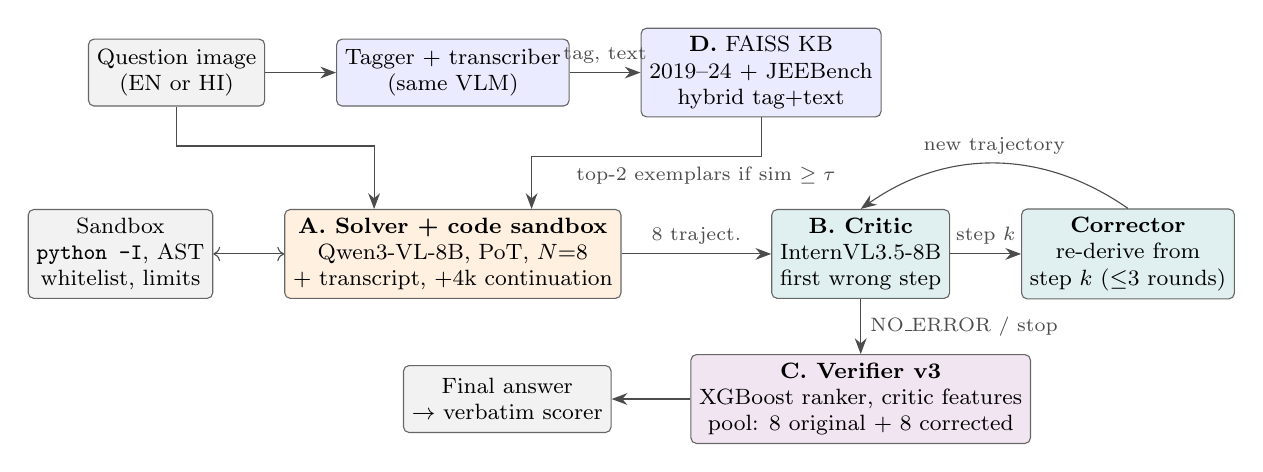
\begin{tikzpicture}[font=\footnotesize, node distance=4mm and 9mm,
  box/.style={draw=black!60, rounded corners=2pt, fill=#1, align=center, minimum height=8.5mm,
  inner sep=3pt}, box/.default=white, arr/.style={-{Stealth[length=2mm]}, black!70}]
\node[box=black!5] (img) {Question image\\(EN or HI)};
\node[box=blue!8, right=of img] (tag) {Tagger + transcriber\\(same VLM)};
\node[box=blue!8, right=of tag] (kb) {\textbf{D.} FAISS KB\\2019--24 + JEEBench\\hybrid tag+text};
\node[box=orange!12, below=13mm of tag, minimum width=34mm] (solver)
  {\textbf{A. Solver + code sandbox}\\Qwen3-VL-8B, PoT, $N{=}8$\\+ transcript, +4k continuation};
\node[box=black!5, left=of solver] (exec) {Sandbox\\\texttt{python -I}, AST\\whitelist, limits};
\node[box=teal!12, right=19mm of solver] (critic) {\textbf{B. Critic}\\InternVL3.5-8B\\first wrong step};
\node[box=teal!12, right=of critic] (corr) {\textbf{Corrector}\\re-derive from\\step $k$ ($\le$3 rounds)};
\node[box=violet!10, below=7mm of critic, minimum width=40mm] (ver)
  {\textbf{C. Verifier v3}\\XGBoost ranker, critic features\\pool: 8 original + 8 corrected};
\node[box=black!5, left=10mm of ver] (out) {Final answer\\$\to$ verbatim scorer};
\draw[arr] (img) -- (tag); \draw[arr] (tag) -- node[above]{\scriptsize tag, text} (kb);
\draw[arr] (kb.south) -- ++(0,-5mm) -| node[pos=0.12,below]{\scriptsize top-2 exemplars if sim $\ge\tau$} ([xshift=10mm]solver.north);
\draw[arr] (img.south) -- ++(0,-5mm) -| ([xshift=-10mm]solver.north);
\draw[arr, <->] (exec) -- (solver);
\draw[arr] (solver) -- node[above]{\scriptsize 8 traject.} (critic);
\draw[arr] (critic) -- node[above]{\scriptsize step $k$} (corr);
\draw[arr] (corr.north) to[bend right=35] node[above]{\scriptsize new trajectory} (critic.north);
\draw[arr] (critic) -- node[right]{\scriptsize NO\_ERROR / stop} (ver);
\draw[arr] (ver) -- (out);
\end{tikzpicture}
\caption{The v3 framework around a frozen VLM. Only the verifier (C) is trained, on
automatically labelled 2019--2024 pools. The v3 changes from v2 are the transcript, the
continuation, hybrid retrieval with JEEBench, and the verifier v3 with its correction gate.}
\label{fig:arch}
\end{figure*}

\textbf{Shared core (v2).} \emph{A. Code sandbox:} the solver writes numbered steps and puts every
calculation in a \texttt{python} block. The block runs in an isolated subprocess (AST whitelist,
no I/O, resource limits), and its output is fed back before generation continues. If no
\verb|\boxed{}| answer appears, a plain-CoT fallback answers.
\emph{B. Correction:} a cross-model critic (InternVL3.5-8B~\cite{internvl35}) names the first
wrong step or says \texttt{NO\_ERROR}. The corrector keeps the earlier steps and re-derives from
the flagged one, for up to 3 rounds; it stops early when the critic accepts the solution or the
answer is unchanged for two rounds.
\emph{C. Verifier:} a classifier over handcrafted and embedding features picks one answer from 16
candidates (8 originals + 8 corrected).
\emph{D. Retrieval:} a one-line concept tag retrieves up to two verified worked solutions from
2019--2024 as exemplars.

\textbf{v3 changes} (Table~\ref{tab:devab}):
(i) \emph{Adaptive budget.} A cut-off answer is continued once for 4{,}096 more tokens. This
applies to every row, including the baselines, so comparisons stay fair.
(ii) \emph{Transcript block.} The solver prompt also contains the VLM's own English
transcription of the question (Hindi is translated), to help it read.
(iii) \emph{RAG v3.} Hybrid tag + problem-text similarity, a KB extended with JEEBench
2016--2018, and $\tau$ tuned by LOYO. LOYO coverage is \RagCovThree\% vs.\ \RagCovTwo\% for the
v2 recipe at the same proxy precision.
(iv) \emph{Verifier v3.} An XGBoost pairwise ranker, selected by LOYO over 2019--2024. It is
trained on pools that, like the test pools, contain corrected solutions, and it gets critic
features (flagged, rounds, answer changed) and agreement over the whole pool and its halves. LOYO
pick accuracy is \VerLoyo\% vs.\ \VerLoyoMaj\% for majority voting (oracle \VerLoyoOracle\%).
(v) \emph{Correction gate.} A chain keeps its corrected answer only if the verifier score rises
by more than $\delta{=}$\GateDelta{}, with $\delta$ chosen out-of-year. This is reported as its
own row; the framework's final answer is still the verifier's pick from the full pool.

\begin{table}[!t]
\centering
\footnotesize
\caption{Dev A/B tests on 2024 (204 questions) that decided the freeze. Rule fixed in advance: include iff $\Delta>0$ and the CI lower bound $>0$.}
\label{tab:devab}
\setlength{\tabcolsep}{3.5pt}
\begin{tabular}{lrrr}
\toprule
Arm & Base & Arm & $\Delta$ [95\% CI] \\
\midrule
Transcript block (PoT) & 50.2 & 55.1 & +4.9 [+1.8, +8.2] \\
Adaptive budget (PoT) & 50.2 & 52.6 & +2.3 [+1.0, +3.7] \\
Adaptive budget (CoT) & 48.5 & 54.9 & +6.4 [+2.5, +10.8] \\
RAG, v2 recipe & 50.2 & 50.4 & +0.2 [$-$2.3, +2.9] \\
RAG v3 (hybrid + JEEBench) & 50.2 & 50.6 & +0.3 [$-$2.1, +3.0] \\
\bottomrule
\end{tabular}
\end{table}


\textbf{Setup.} Qwen3-VL-8B-Instruct~\cite{qwen3vl} and InternVL3.5-8B (AWQ 4-bit) run with
vLLM~\cite{vllm} on one RTX 3060, one model at a time. Sampling uses $T{=}0.7$, top-$p$ 0.8 and
top-$k$ 20, the same for all rows. CoT takes 20 samples per question; PoT and correction take 8.
Every call is cached in SQLite and seeds are deterministic, so the three lab shutdowns during the
final batch resumed without changing any result.

% ----------------------------------------------------------------------------------------------
\section{Results on the clean 2026 test}
\begin{table*}[!t]
\centering
\footnotesize
\caption{Table~I on the clean 2026 test set (204 questions). Top: frozen v3 framework. Bottom: the frozen v2 framework re-run unchanged. Accuracy in \%; 95\% cluster-bootstrap CIs over EN/HI twins; tokens are generated tokens.}
\label{tab:t26}
\setlength{\tabcolsep}{3.5pt}
\begin{tabular}{lrrrrrr}
\toprule
Configuration & Acc. & Num. & 95\% CI & $\Delta$ vs.\ baseline [CI] & Tok./q & Calls/q \\
\midrule
\multicolumn{7}{l}{\emph{v3 framework}} \\
Baseline (single-pass CoT, adaptive budget) & 44.3 & 29.5 & 37.4--51.0 & -- & 4.5k & 1.0 \\
Self-consistency (matched compute) ($n{=}18$) & 52.5 & 34.6 & 43.1--61.3 & +8.2 [+4.5, +12.0] & 80.4k & 18.0 \\
+ Code sandbox + RAG v3 + transcript (v3 PoT) & 49.8 & 37.3 & 42.5--56.9 & +5.6 [+2.0, +9.2] & 6.5k & 2.2 \\
+ Learned verifier v3 (PoT pool only) & 57.8 & 41.0 & 48.5--66.2 & +13.6 [+8.4, +18.6] & 51.8k & 18.3 \\
+ Correction (cross-model critic) & 52.0 & 39.6 & 44.6--59.2 & +7.7 [+4.3, +11.0] & 10.0k & 5.1 \\
+ Correction (gated) & 52.6 & 39.9 & 44.9--60.1 & +8.3 [+4.7, +11.7] & 10.0k & 5.1 \\
v3 framework (verifier v3) & \textbf{58.8} & 44.9 & 50.0--67.2 & +14.6 [+9.6, +19.5] & 80.3k & 41.7 \\
\midrule
\multicolumn{7}{l}{\emph{v2 framework (re-run)}} \\
Baseline (single-pass CoT) & 41.2 & 26.5 & 34.4--47.9 & -- & 2.9k & 1.0 \\
Self-consistency (matched compute) ($n{=}20$, needs 21) & 49.0 & 28.2 & 40.2--57.4 & +7.8 [+4.4, +11.3] & 58.0k & 20.0 \\
+ Code sandbox & 43.0 & 31.1 & 36.4--49.6 & +1.8 [$-$1.1, +4.7] & 4.0k & 1.8 \\
+ Agentic correction (cross-model critic) & 46.8 & 36.2 & 40.1--53.4 & +5.5 [+2.1, +9.0] & 7.4k & 4.7 \\
+ Learned verifier & 55.4 & 39.7 & 46.6--63.7 & +14.2 [+9.0, +19.5] & 59.2k & 38.0 \\
Full framework & \textbf{55.4} & 39.7 & 46.6--63.7 & +14.2 [+9.0, +19.3] & 60.1k & 38.8 \\
\bottomrule
\end{tabular}
\end{table*}


\subsection{Main result}
Table~\ref{tab:t26} and Fig.~\ref{fig:t26} give the SOP's Table~I for both frameworks. The v3 framework
reaches \textbf{\ThreeAcc\%} vs.\ \ThreeBase\% for single-pass CoT (\ThreeGain{} points). At
\ThreeTok{} generated tokens per question, matched SC uses \ThreeScN{} samples and reaches
\ThreeSc\%. The framework is \ThreeVsSc{} points better (CI [\ThreeVsScLo, \ThreeVsScHi]): it
answers \ThreeFwOnly{} questions that SC misses, against \ThreeScOnly{} the other way. The frozen
v2 framework reaches \TwoAcc\%, also \TwoVsSc{} points above its matched SC (CI
[\TwoVsScLo, \TwoVsScHi], $p{=}$\TwoVsScP). \emph{The main v2 claim, beating compute-matched
self-consistency, therefore holds on an exam the model cannot have seen.} Fig.~\ref{fig:compute}
shows that every framework row lies above the SC curve at its cost.

\begin{figure}[t]
\centering
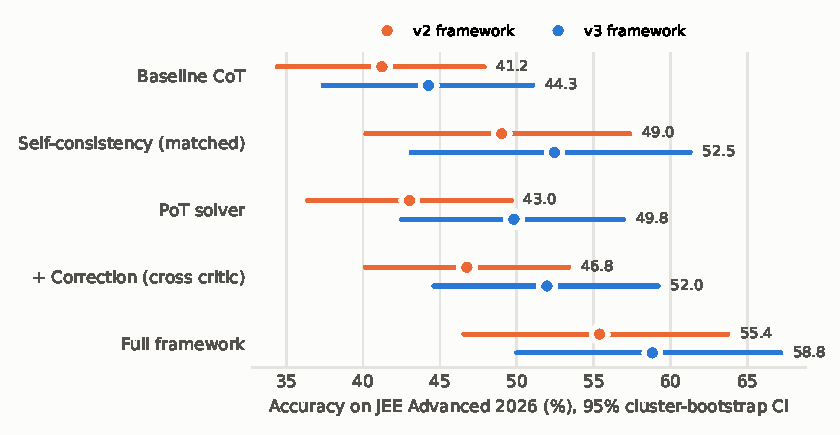
\includegraphics[width=\columnwidth]{table1_2026.pdf}
\caption{2026 clean test: matching rows of the v2 and v3 frameworks, with 95\% cluster-bootstrap
CIs.}
\label{fig:t26}
\end{figure}

\begin{figure}[t]
\centering
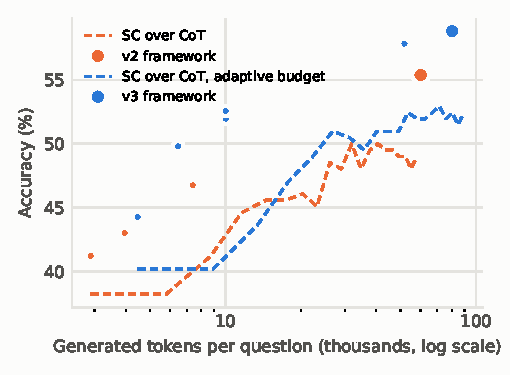
\includegraphics[width=\columnwidth]{compute_2026.pdf}
\caption{2026: accuracy vs.\ generated tokens. Dashed: SC over $n$ CoT samples (majority vote).
Dots: Table~I rows; large dots: the full frameworks.}
\label{fig:compute}
\end{figure}

\subsection{v3 vs.\ v2}
\begin{table}[!t]
\centering
\scriptsize
\caption{Paired comparisons (cluster bootstrap; McNemar counts questions only $a$ / only $b$ gets right; it is meaningful for single-answer rows only, as Pass@1 rows are rounded per question). $^\dagger$post-hoc.}
\label{tab:cmp}
\setlength{\tabcolsep}{2.5pt}
\begin{tabular}{lrrrr}
\toprule
Comparison ($a$ vs.\ $b$) & $\Delta$ [95\% CI] & P($\Delta{\le}0$) & $a$/$b$ & $p$ \\
\midrule
2026 v3 fw vs.\ v2 fw & +3.4 [$-$1.5, +8.8] & 0.113 & 16/9 & 0.230 \\
2026 v3 PoT vs.\ v2 PoT & +6.8 [+3.6, +10.0] & 0.000 & 27/3 & $<$0.001 \\
2026 CoT adaptive budget vs.\ CoT & +3.0 [+1.7, +4.5] & 0.000 & 6/3 & 0.508 \\
2026 gated vs.\ ungated correction (v3) & +0.6 [$-$0.4, +1.5] & 0.122 & 4/1 & 0.375 \\
2026 verifier v3 pick vs.\ v3 PoT mean & +9.0 [+5.8, +12.4] & 0.000 & 17/0 & $<$0.001 \\
2025$^\dagger$ v3 fw vs.\ v2 fw & +6.8 [+1.1, +12.1] & 0.012 & 21/8 & 0.024 \\
2025$^\dagger$ v3 PoT vs.\ v2 PoT & +8.1 [+4.8, +11.6] & 0.000 & 30/7 & $<$0.001 \\
\bottomrule
\end{tabular}
\end{table}

Table~\ref{tab:cmp} gives the paired tests. The v3 solver is clearly better: v3 PoT beats v2 PoT
by \PotVsDiff{} points (CI [\PotVsLo, \PotVsHi]). The adaptive budget alone lifts CoT by
\ExtVsDiff. The full v3 framework is \VsDiff{} points above v2 (CI [\VsLo, \VsHi],
$p{=}$\VsP), which is \emph{not} significant on \NTest{} questions. On the post-hoc 2025 set the
same comparison is \PostVsDiff{} (CI [\PostVsLo, \PostVsHi]). The difference between the two
years is largely the verifier (Sec.~\ref{sec:ver}).

\subsection{Where the frameworks win and lose}
\begin{table}[!t]
\centering
\footnotesize
\caption{Full-framework accuracy (\%) by group. 2025 is post-hoc.}
\label{tab:bd}
\setlength{\tabcolsep}{3.5pt}
\begin{tabular}{lrrrr}
\toprule
Group & v2 '26 & v3 '26 & v2 '25 & v3 '25 \\
\midrule
English & 60.8 & 63.7 & 73.7 & 74.7 \\
Hindi & 50.0 & 53.9 & 56.8 & 69.5 \\
Text only & 69.6 & 72.5 & 72.5 & 81.9 \\
Needs image & 25.8 & 30.3 & 46.2 & 46.2 \\
Physics & 32.4 & 35.3 & 54.8 & 64.5 \\
Chemistry & 52.9 & 60.3 & 60.9 & 59.4 \\
Mathematics & 80.9 & 80.9 & 79.7 & 92.2 \\
MCQ-Single & 79.2 & 83.3 & 67.4 & 65.2 \\
MCQ-Multiple & 55.6 & 55.6 & 59.5 & 69.0 \\
Numerical & 39.7 & 44.9 & 69.0 & 77.4 \\
Matching & 58.3 & 62.5 & 55.6 & 72.2 \\
\bottomrule
\end{tabular}
\end{table}

Table~\ref{tab:bd} shows that v3 improves on most groups, but the gaps the paper reports remain.
For v3 on 2026, English reaches \ThreeEn\% and Hindi \ThreeHin\%; text-only questions reach
\ThreeTxt\% and diagram questions only \ThreeImg\%. Inference-time reasoning does not fix
perception. Part of the Hindi gap on 2026 may come from our own crops.

\subsection{Correction loop and the correction gate}
\begin{table}[!t]
\centering
\scriptsize
\caption{Correction loop, paper-style metacognition (\%). EP: wrong solutions flagged in round 1; EC: round-1 fixes among detected; FA: correct solutions flagged. W$\to$R / R$\to$W: answer flips after all rounds.}
\label{tab:corr}
\setlength{\tabcolsep}{2.5pt}
\begin{tabular}{lrrrrrrr}
\toprule
Run & Chains & Acc. & EP & EC & FA & W$\to$R & R$\to$W \\
\midrule
2026 pot\_corr\_cross & 1632 & 43.0$\to$46.8 & 67.5 & 9.7 & 23.6 & 76 & 15 \\
2026 full & 1632 & 44.7$\to$48.8 & 69.0 & 10.8 & 25.2 & 83 & 16 \\
2026 v3\_full & 1632 & 49.8$\to$52.0 & 52.9 & 13.2 & 19.9 & 68 & 33 \\
2025 v3\_full & 1520 & 56.2$\to$57.9 & 40.3 & 13.1 & 23.3 & 46 & 21 \\
2025 pot\_corr\_cross (v2) & 1520 & 48.2$\to$51.3 & 59.3 & 13.3 & 25.7 & 87 & 39 \\
2025 full (v2) & 1520 & 50.9$\to$54.7 & 60.7 & 15.7 & 28.6 & 87 & 29 \\
\bottomrule
\end{tabular}
\end{table}

\begin{table}[!t]
\centering
\footnotesize
\caption{Correction gate: per-chain accuracy (\%) and flips, ungated $\to$ gated.}
\label{tab:gate}
\setlength{\tabcolsep}{3.5pt}
\begin{tabular}{lrrrrrr}
\toprule
Set & Chains & Orig. & Corr. & Gated & W$\to$R & R$\to$W \\
\midrule
Train (LOYO, picks $\delta$) & 1936 & 44.4 & 47.6 & \textbf{48.2} & 95$\to$88 & 32$\to$14 \\
2026 (clean) & 1632 & 49.8 & 52.0 & \textbf{52.6} & 68$\to$54 & 33$\to$9 \\
2025 (post-hoc) & 1520 & 56.2 & 57.9 & \textbf{58.5} & 46$\to$41 & 21$\to$7 \\
\bottomrule
\end{tabular}
\end{table}

In the paper's terms (Table~\ref{tab:corr}), the cross-model critic flags \EpThree\% of wrong v3
solutions in round 1 (\EpTwo\% for v2). Round-1 correction fixes \EcThree\% of the detected errors
(\EcTwo\% for v2), well above the paper's 1.1--5.2\% single-pass rate. The critic also flags
\FaThree\% of \emph{correct} solutions. Because the v3 solver is stronger, fewer wrong solutions
remain, and the correction loop gains less in absolute terms.

The gate (Table~\ref{tab:gate}) does what it was trained for. On 2026 it cuts right$\to$wrong
flips from \GateRtwU{} to \GateRtwG{} while keeping most fixes (\GateWtrU$\to$\GateWtrG{}
wrong$\to$right). Per-chain accuracy goes from \GateAccU\% to \GateAccG\% (\GateVsDiff{}, CI
[\GateVsLo, \GateVsHi]); the change is small and not significant. The flip pattern carries over
from the training years to both test years.

\subsection{Verifier: classifier vs.\ selector}\label{sec:ver}
\begin{table}[!t]
\centering
\footnotesize
\caption{Primary verifier on its own 16-answer test pool: AUC and accuracy of the picked answer vs.\ pool baselines (\%).}
\label{tab:ver}
\setlength{\tabcolsep}{3.5pt}
\begin{tabular}{llrrrrr}
\toprule
Pool & Verifier & AUC & Pick & Maj. & Rand. & Oracle \\
\midrule
2026 v3 & xgb\_ranker/handcrafted & 0.902 & \textbf{58.8} & 59.3 & 50.9 & 79.4 \\
2026 v2 & logreg/all & 0.913 & \textbf{55.4} & 53.9 & 46.7 & 76.5 \\
2025 v3 & xgb\_ranker/handcrafted & 0.872 & \textbf{72.1} & 65.8 & 57.1 & 87.4 \\
2025 v2 & logreg/all & 0.836 & \textbf{65.3} & 65.8 & 52.8 & 85.3 \\
\bottomrule
\end{tabular}
\end{table}

As a classifier, verifier v3 transfers well: its AUC on the 2026 pool is \VerAucTest{}.
\emph{As a selector, on the clean year, it adds nothing}: it picks \ThreePick\% vs.\ \ThreeMaj\%
for majority voting over the same 16 answers (\ThreePickVsMaj), with an oracle of
\ThreeOracle\%. On 2025 it beats majority by \PostPickVsMaj{} points. So the v3 gain on 2026 comes
from a better candidate pool (transcript, continuation, correction), not from selection. Picking
among the 8 PoT samples alone already reaches \ThreePotVer\%.

The shift stated before the runs is visible in Table~\ref{tab:shift}. The verifier was trained on
plain PoT solutions of about \TokTrain{} tokens (\TruncTrain\% cut off). The 2026 v3 solutions are
\TokTest{} long because of the transcript and continuation, and \TruncTest\% are cut off. This is a
plausible reason the selector gain does not carry over to the clean year.

\begin{table}[!t]
\centering
\scriptsize
\caption{Shift between the verifier's training solutions and the test pools. Cut: \texttt{finish = length} on the final call.}
\label{tab:shift}
\setlength{\tabcolsep}{2.5pt}
\begin{tabular}{lrrrrrr}
\toprule
Solutions & Rows & Acc. & Cut & Tok. & Acc.\,cut & Acc.\,compl. \\
\midrule
train 2019-2024 pot\_train & 10160 & 45.5 & 37.2 & 3.5k & 28.9 & 55.3 \\
2026 pot & 1632 & 43.0 & 42.8 & 4.0k & 27.0 & 55.0 \\
2026 v3\_pot & 1632 & 49.8 & 40.3 & 6.5k & 32.0 & 61.8 \\
2025 pot & 1520 & 48.2 & 36.7 & 3.5k & 29.9 & 58.7 \\
2025 v3\_pot & 1520 & 56.2 & 36.6 & 5.9k & 41.7 & 64.7 \\
\bottomrule
\end{tabular}
\end{table}


% ----------------------------------------------------------------------------------------------
\section{Post-hoc 2025, model bridge and memorisation}
\begin{table*}[!t]
\centering
\footnotesize
\caption{v3 Table~I on 2025 (190 questions, \textbf{post-hoc}: 2025 was used to pilot v1/v2).}
\label{tab:t25}
\setlength{\tabcolsep}{3.5pt}
\begin{tabular}{lrrrrrr}
\toprule
Configuration & Acc. & Num. & 95\% CI & $\Delta$ vs.\ baseline [CI] & Tok./q & Calls/q \\
\midrule
Baseline (single-pass CoT, adaptive budget) & 48.3 & 43.2 & 41.7--55.3 & -- & 4.0k & 1.0 \\
Self-consistency (matched compute) ($n{=}18$) & 58.4 & 52.4 & 50.0--66.8 & +10.1 [+6.1, +14.1] & 72.4k & 18.0 \\
+ Code sandbox + RAG v3 + transcript (v3 PoT) & 56.2 & 59.7 & 49.5--63.0 & +8.0 [+3.3, +13.1] & 5.9k & 2.3 \\
+ Learned verifier v3 (PoT pool only) & 68.9 & 72.6 & 61.1--76.8 & +20.7 [+14.7, +27.3] & 47.3k & 19.5 \\
+ Correction (cross-model critic) & 57.9 & 62.5 & 51.1--64.5 & +9.6 [+4.8, +15.0] & 8.7k & 5.0 \\
+ Correction (gated) & 58.5 & 63.7 & 51.7--65.1 & +10.2 [+5.3, +15.6] & 8.7k & 5.0 \\
v3 framework (verifier v3) & \textbf{72.1} & 77.4 & 64.7--80.5 & +23.8 [+17.4, +30.7] & 69.9k & 41.1 \\
\bottomrule
\end{tabular}
\end{table*}

\textbf{2025 (post-hoc).} The v3 framework reaches \PostAcc\% (Table~\ref{tab:t25}) vs.\
\PostTwoAcc\% for the frozen v2 run, and beats matched SC by \PostVsSc{} points. Since 2025 shaped
earlier design choices and may be in the model's training data, we do not base claims on it. The
larger gaps on 2025 than on 2026 are consistent with some optimism on that year.

\begin{table*}[!t]
\centering
\footnotesize
\caption{Bridge: the framework with the paper's Qwen2.5-VL-7B on 2025 (clean for that model; verifier transferred from Qwen3).}
\label{tab:q25}
\setlength{\tabcolsep}{3.5pt}
\begin{tabular}{lrrrrrr}
\toprule
Configuration & Acc. & Num. & 95\% CI & $\Delta$ vs.\ baseline [CI] & Tok./q & Calls/q \\
\midrule
Baseline (single-pass CoT) & 14.0 & 6.6 & 11.0--17.3 & -- & 0.7k & 1.0 \\
Self-consistency (matched compute) ($n{=}20$, needs 33) & 16.3 & 10.7 & 10.0--23.2 & +2.3 [$-$1.9, +6.5] & 14.1k & 20.0 \\
+ Code sandbox & 13.9 & 5.7 & 10.2--18.0 & $-$0.1 [$-$2.9, +2.9] & 1.0k & 3.6 \\
+ Correction (same-model critic) & 13.9 & 6.1 & 10.2--17.9 & $-$0.1 [$-$2.9, +2.9] & 1.5k & 6.7 \\
+ Correction (cross-model critic) & 13.7 & 8.0 & 10.3--17.3 & $-$0.3 [$-$2.9, +2.5] & 2.8k & 11.6 \\
+ Learned verifier (transfer) & 15.3 & 8.3 & 10.0--21.1 & +1.3 [$-$3.3, +6.0] & 22.7k & 92.9 \\
\bottomrule
\end{tabular}
\end{table*}

\textbf{Bridge to the paper's model.} With Qwen2.5-VL-7B (2025 is clean for this model), the
framework does not help: \QBase\% for CoT, \QSc\% for matched SC and \QFull\% for the framework
(\QVsSc{} vs.\ SC, CI [\QVsScLo, \QVsScHi]; Table~\ref{tab:q25}). At about 14\% accuracy, most
candidates are wrong, so agreement, critique and verification carry little signal. The framework
needs a solver that is right often enough.

\begin{table}[!t]
\centering
\footnotesize
\caption{Memorisation probe: answer-only accuracy (\%, 64 tokens) by exam year. 2026 is after both models' release.}
\label{tab:probes}
\setlength{\tabcolsep}{3.5pt}
\begin{tabular}{lrrrrrrrr}
\toprule
Model & '19 & '20 & '21 & '22 & '23 & '24 & '25 & '26 \\
\midrule
Qwen3-VL-8B & 12.5 & 14.6 & 11.8 & 10.5 & 14.5 & 15.7 & 13.2 & 15.2 \\
Qwen2.5-VL-7B & 12.5 & 12.3 & 14.5 & 17.1 & 13.5 & 14.2 & 12.1 & 21.1 \\
\bottomrule
\end{tabular}
\end{table}

\textbf{Memorisation probes.} Asked for the answer only, Qwen3-VL scores \ProbeOldLo--\ProbeOldHi\%
on 2019--2024, \ProbeTwentyFive\% on 2025 and \ProbeTwentySix\% on the clean 2026
(Table~\ref{tab:probes}). The clean year is not lower, so we see no memorisation signal. Pass@5 of
v3 PoT on 2026 is \PassFiveThree\%, well above any selector, so there is
still headroom in the pool.

% ----------------------------------------------------------------------------------------------
\section{Post-hoc extensions (Phase 4)}\label{sec:v4}
After the v3 result we tried to fix its two weak points, selection and retrieval. Both test years
had been seen by then, so \emph{every Phase-4 number on 2025 or 2026 is post-hoc}. All choices
used 2019--2024 only, and a second pre-registration (\texttt{V4\_PREREG.md}), written before any
Phase-4 scoring, fixed the rules: a new selector is scored on the test years only if its LOYO
accuracy beats the v3 ranker's on every pool kind. The v3 result above stays the headline.

\textbf{Diagnosis.} Length shift is not the main cause of the 2026 selector failure. v3 solutions
are longer than the training pools in \emph{both} years (\VfTokTwentyFive{} and \VfTokTwentySix{}
vs.\ \VfTokTrain{} tokens), with small standardised shifts of log length (\VfSmdTwentyFive{} and
\VfSmdTwentySix). Yet the verifier beats majority on 2025 (\VfVerMajTwentyFive) and not on 2026
(\VfVerMajTwentySix). On 2026 it loses mainly on pools that are mostly finished (\VfFinVer\% vs.\
\VfFinMaj\%). Of the 2026 errors, \VfErrMiss{} are selector misses and \VfErrNever{} never had a
right answer in the pool. In the selector-miss pools only \VfErrShare\% of candidates are right,
so the right answer is a small minority. Diagram questions dominate: \VfImgMiss\% of them are
selector misses, vs.\ \VfTxtMiss\% of text-only questions.

\begin{table}[!t]
\centering
\scriptsize
\caption{Phase~4 selectors, LOYO selection accuracy (\%) on 2019--2024 (no test data). \emph{v3 pools}: the 16-answer training pools of verifier v3; \emph{+W2}: retrained with the new v3-style pools (S5), evaluated on the v3 pools and on the new pools. Each run uses its best of max-prob / weighted / log-odds vote on the v3 pools (Method: base run). Gate (fixed in advance): beat the v3 ranker on every pool kind.}
\label{tab:v4sel}
\setlength{\tabcolsep}{2.5pt}
\begin{tabular}{lrrrlr}
\toprule
Selector & v3 pools & +W2: v3 & +W2: new & Method & Gate \\
\midrule
v3 ranker (refit) & 62.0 & 61.2 & 59.5 & max-prob & ref. \\
S2 no length & 59.1 & 61.6 & 60.1 & log-odds & fail \\
S3 neural & 57.0 & 58.7 & 56.8 & weighted & fail \\
S4 stacked & 60.3 & 61.2 & 58.8 & max-prob & fail \\
\midrule
Majority vote & 53.7 & 53.7 & 55.8 &  &  \\
Oracle & 78.5 & 78.5 & 71.6 &  &  \\
\bottomrule
\end{tabular}
\end{table}


\textbf{Selectors} (Table~\ref{tab:v4sel}, Fig.~\ref{fig:v4sel}). All of these were chosen by LOYO:
\begin{itemize}
\item \emph{S2:} the v3 ranker without its length features.
\item \emph{S3:} a neural verifier. This is a ModernBERT-base cross-encoder~\cite{modernbert},
fine-tuned on (English transcript, answer, solution tail; 1{,}024 tokens) with one fold per
training year.
\item \emph{S4:} the v3 ranker with the neural score as an extra feature.
\item \emph{S5:} S2--S4 retrained with \VfXRows{} new v3-style training candidates (398 training
questions, 4 PoT samples each plus their corrections; about 30 GPU-hours). The training pools
then match the test-time solutions.
\end{itemize}
None passes its gate. The neural verifier does learn a signal: candidate AUC is \VfAuc{}
(\VfAucLo--\VfAucHi{} by year), and as a vote weight it beats majority (\VfNeural\% vs.\ \VfMaj\%).
But it ranks worse than the handcrafted ranker (\VfRef\%). Dropping the length features costs
accuracy (\VfNoLen\%), consistent with the diagnosis. Matched pools do not help either: the
ranker refit with them reaches \VfXRef\%, within the noise of about 1 point we measured for
ranker LOYO on these 242 pools. As pre-registered, no Phase-4 selector is scored on test. The
one-shot evaluation reproduces the v3 selector (\VfSZero\%) and majority (\VfSOne\%) on 2026.

\begin{figure}[t]
\centering
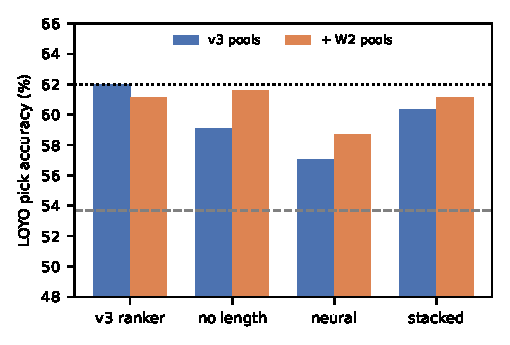
\includegraphics[width=0.92\columnwidth]{v4_selectors.pdf}
\caption{Phase~4 selectors: LOYO pick accuracy on the 16-answer training pools, trained on the
v3 pools or with the new v3-style pools added. Dotted: the v3 ranker; dashed: majority vote.}
\label{fig:v4sel}
\end{figure}

\begin{table}[!t]
\centering
\scriptsize
\caption{RAG in Phase~4, paired differences (points, 95\% cluster-bootstrap CI). Top: 2024 dev year with matched seeds, 204 questions, RAG fires on 31. Bottom: post-hoc 2026 PoT with the extended KB ($^\dagger$right column: questions whose retrieval changed). LOYO coverage at proxy precision 0.70: kb\_v4 13.5\% vs.\ kb\_v3 15.0\%.}
\label{tab:v4rag}
\setlength{\tabcolsep}{2.5pt}
\begin{tabular}{lrr}
\toprule
Comparison & All & RAG fires \\
\midrule
Solutions $-$ no RAG & $-$0.2 [$-$1.0, +0.4] & $-$1.6 [$-$6.2, +2.5] \\
Cards $-$ no RAG & +0.3 [$-$0.2, +0.9] & +2.0 [$-$1.6, +6.2] \\
\textbf{Cards $-$ solutions} & +0.6 [$-$0.1, +1.3] & +3.6 [$-$0.8, +8.5] \\
\midrule
kb\_v4 $-$ kb\_v3, 2026$^\dagger$ & +0.0 [$-$0.4, +0.4] & +0.0 [$-$6.2, +7.3] \\
\bottomrule
\end{tabular}
\end{table}


\textbf{Retrieval} (Table~\ref{tab:v4rag}).
\begin{itemize}
\item \emph{Matched seeds.} RAG runs now reuse the no-RAG sampling seeds. A question without
exemplars therefore gets identical outputs, and the RAG effect is measured only where RAG fires
(\VfFired{} of \VfDevQ{} dev questions).
\item \emph{Method cards.} The worked-solution exemplar is replaced by a short card: method, when
it applies, plan, key equations and a common mistake, with the answer removed. On the 2024 dev
year, where RAG fires, cards beat solution exemplars by \VfCardSol{} points
(P($\Delta{\le}0$)${=}$\VfCardSolP). The lower bound is below zero, so by the inclusion rule cards
are not adopted.
\item \emph{Open-licensed KB.} We added \VfOlyEntries{} verified OlympiadBench~\cite{olympiadbench}
solutions (Apache-2.0; text-only, numeric answers). LOYO coverage at proxy precision 0.70 falls
from \VfCovThree\% to \VfCovFour\%: the new near neighbours raise the tuned threshold, and they
give only \VfOlyHits{} hits themselves. On 2026, retrieval changes for \VfKbChanged{} questions,
and PoT accuracy is unchanged (\VfKbAll). Coaching material was ruled out for licensing and
leakage reasons.
\item \emph{Mixed pools.} Half-RAG, half-plain pools give \VfMixed\% majority-vote accuracy on
2026 vs.\ \VfMixRag\% (RAG) and \VfMixPot\% (plain).
\end{itemize}

\textbf{Takeaway.} Each Phase-4 idea addressed a measured weakness and was tested by a rule fixed
in advance. None improves on v3. The 2026 selection gap is not explained by length shift. A
stronger learned verifier does not close it, and neither do matched training pools. Most
remaining errors are perception failures on diagram questions, where the right answer is rare or
absent in the pool.

% ----------------------------------------------------------------------------------------------
\section{Discussion}
\textbf{What holds on clean data.} Code-based sampling, cross-model correction and selection beat
voting on plain CoT at the same cost, for both v2 and v3. The transcript block and the adaptive
budget give a significantly stronger solver.

\textbf{What does not.} Verifier v3 beat majority voting under LOYO and on 2025, but not on 2026.
Its features shift with the longer v3 solutions, and its selector gain does not survive the
change. Phase~4 shows this is not simply length shift: a fine-tuned neural verifier, a ranker
without length features and pools matched to the v3 solutions all stay below the v3 ranker under
LOYO. The correction gate removes most harmful flips but barely moves accuracy. Retrieval stays a
small effect; method cards are a promising but unconfirmed trend.

\textbf{Remaining failures.} Diagram questions and Hindi questions still lag far behind, and
about two in five PoT trajectories still end cut off.

\section{Limitations}
One substrate model; one clean year of \NTest{} questions (CIs about $\pm$8 points), so
differences of a few points are not resolvable. The Hindi 2026 crops are our own. The transcript
and the KB texts come from the same VLM. Compute matching counts generated tokens, not prompt
tokens or code execution. Phase-4 numbers on 2025 and 2026 are post-hoc, and its dev A/Bs have
only about 30 questions where RAG fires.

\section{Conclusion}
On an exam year the model cannot have seen, a frozen 8B VLM with a code sandbox, cross-model
correction and answer selection improves accuracy from \ThreeBase\% to \ThreeAcc\% and beats
compute-matched self-consistency by \ThreeVsSc{} points. The v2 framework's claim reproduces on
the clean year (\TwoVsSc). v3's pre-registered changes make the solver stronger, but its total
advantage over v2 is not significant, and its verifier does not beat majority voting there.
Phase~4 rules out the obvious fixes on the selection side. The next steps are better perception
for diagrams and Hindi, which would put the right answer into more pools, and larger dev sets to
test retrieval changes such as method cards.

\section*{Reproducibility}
Code, configs and tests are in \texttt{mmjee-reasoner/}. The frozen v3 config is
\texttt{configs/v3\_final.yaml} (\texttt{V3\_FREEZE.md}). Evaluation uses
\texttt{configs/v3\_eval.yaml} and \texttt{configs/v3\_eval\_v2fw.yaml}, and
\texttt{scripts/final\_report\_v3.py} regenerates every v3 table, macro and figure. Phase~4 is
isolated in \texttt{artifacts\_v4/} and \texttt{configs/v4*.yaml} (\texttt{V4\_PREREG.md},
\texttt{docs/phases/PHASE4.md}); \texttt{scripts/v4\_eval.py} is the
one-shot test evaluation and \texttt{scripts/final\_report\_v4.py} writes Sec.~\ref{sec:v4}.

\begin{thebibliography}{99}\footnotesize
\bibitem{mmjee} A.~Mukherjee and S.~Ghosh, ``mmJEE-Eval: A bilingual multimodal benchmark for
evaluating scientific reasoning in vision-language models,'' in \emph{Proc.\ IJCNLP-AACL}, 2025.
\bibitem{selfconsistency} X.~Wang \emph{et al.}, ``Self-consistency improves chain of thought
reasoning in language models,'' in \emph{Proc.\ ICLR}, 2023.
\bibitem{pot} W.~Chen \emph{et al.}, ``Program of thoughts prompting: Disentangling computation
from reasoning for numerical reasoning tasks,'' \emph{TMLR}, 2023.
\bibitem{pal} L.~Gao \emph{et al.}, ``PAL: Program-aided language models,'' in \emph{Proc.\
ICML}, 2023.
\bibitem{selfrefine} A.~Madaan \emph{et al.}, ``Self-Refine: Iterative refinement with
self-feedback,'' in \emph{Proc.\ NeurIPS}, 2023.
\bibitem{critic} Z.~Gou \emph{et al.}, ``CRITIC: Large language models can self-correct with
tool-interactive critiquing,'' in \emph{Proc.\ ICLR}, 2024.
\bibitem{cannotselfcorrect} J.~Huang \emph{et al.}, ``Large language models cannot self-correct
reasoning yet,'' in \emph{Proc.\ ICLR}, 2024.
\bibitem{cobbe} K.~Cobbe \emph{et al.}, ``Training verifiers to solve math word problems,''
arXiv:2110.14168, 2021.
\bibitem{lightman} H.~Lightman \emph{et al.}, ``Let's verify step by step,'' in \emph{Proc.\
ICLR}, 2024.
\bibitem{rag} P.~Lewis \emph{et al.}, ``Retrieval-augmented generation for knowledge-intensive
NLP tasks,'' in \emph{Proc.\ NeurIPS}, 2020.
\bibitem{faiss} J.~Johnson, M.~Douze and H.~J\'egou, ``Billion-scale similarity search with
GPUs,'' \emph{IEEE Trans.\ Big Data}, 2019.
\bibitem{bge} S.~Xiao \emph{et al.}, ``C-Pack: Packed resources for general Chinese
embeddings,'' in \emph{Proc.\ SIGIR}, 2024.
\bibitem{vllm} W.~Kwon \emph{et al.}, ``Efficient memory management for large language model
serving with PagedAttention,'' in \emph{Proc.\ SOSP}, 2023.
\bibitem{qwen3vl} Qwen Team, ``Qwen3-VL,'' model release and technical report, 2025.
\bibitem{internvl35} OpenGVLab, ``InternVL3.5,'' model release and technical report, 2025.
\bibitem{modernbert} B.~Warner \emph{et al.}, ``Smarter, better, faster, longer: A modern
bidirectional encoder for fast, memory efficient, and long context finetuning and inference''
(ModernBERT), arXiv:2412.13663, 2024.
\bibitem{olympiadbench} C.~He \emph{et al.}, ``OlympiadBench: A challenging benchmark for
promoting AGI with Olympiad-level bilingual multimodal scientific problems,'' in \emph{Proc.\
ACL}, 2024.
\end{thebibliography}
\end{document}
